To verify the functional correctness of graph
algorithms we need a framework to reason about mathematical graphs.
As will be shown in \S\ref{sec:development}, our mathematical
graph constructions comprise a considerable fraction of our
codebase.  Indeed, as discussed in \S\ref{sec:related},
25 years of research into mechanized graph theory can
be summarized as ``it is a little tricky''.  While
we have some elegant definitions and proofs,
our two key contributions for this section are more abstract.

First, as demonstrated in \S\ref{sec:orientation},
our development is expressive and powerful enough to verify realistic
algorithms---that is, it actually works in an end-to-end system.
Second, we have taken considerable care to develop a modular and
general-purpose framework for such mathematical graphs to allow
such verifications to be mechanized without undue pain.
Accordingly, in this section we will present our framework
at a high level to communicate the overall architecture rather
than focusing on the nitty-gritty details.

\subsection{Structure of the mathematical graph framework}\label{sec:mathinfra}

\begin{figure}[htbp]
\centering
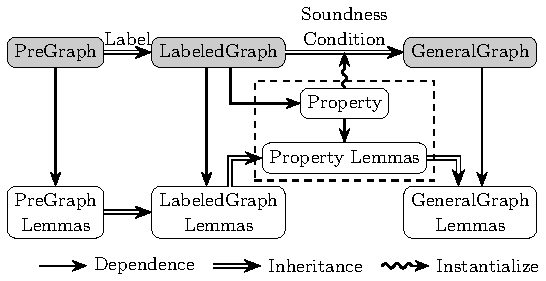
\includegraphics{variousgraph.pdf}
\caption{Structure of the Mathematical Graph Library}\label{fig:graphs}
\end{figure}

Figure~\ref{fig:graphs} gives the overall architecture of our mathematical graph library. The most basic kind of graph is PreGraph, out of which we build LabeledGraphs, and which in turn are used
to build GeneralGraphs.  Each kind has some lemmas and also inherits the lemmas of the previous kind.  The dashed box represents a ``plugin'' system for attaching arbitrary properties to LabeledGraphs (\ref{subsec:graphplugins}). %and will be discussed later. %We will consider each in turn.

\begin{figure}[htbp]
\centering
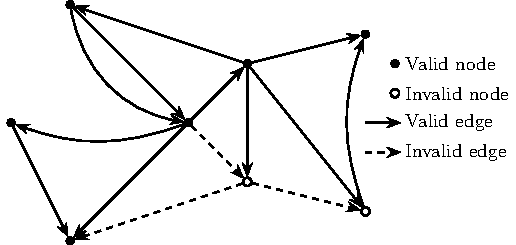
\includegraphics{pregraphexp.pdf}
\caption{A PreGraph with invalid nodes and edges.}\label{fig:pregraph}
\end{figure}

\vspace{-0.75ex}
%%%%%%%%%%%%%%%%%%%%%%%%%%%%%%%%%%%%%%%%%%%%%%%%%%
%%%%%% Edit 1
%%%%%%%%%%%%%%%%%%%%%%%%%%%%%%%%%%%%%%%%%%%%%%%%%%
%%%%%% Edit 1: Qinxiang's proposal starts
%%%%%%%%%%%%%%%%%%%%%%%%%%%%%%%%%%%%%%%%%%%%%%%%%%
\iftrue
\paragraph{Pregraphs.} A PreGraph is a hextuple $(V, E, \phi_V, \phi_E, s, d)$,
where $V$ and $E$ are the underlying carrier sets of vertices and edges.  Not every $v \in V$ or $e \in E$ is actually ``in'' the graph, so we provide the predicates $\phi_V$ and $\phi_E$ to classify vertices and edges as \emph{valid} (in) or not (out).  Finally, $s$ and $d : E -> V$ are functions that map an edges to their source and destination respectively; this model means that PreGraphs are directed rather than undirected.  By design, there are no requirements for \emph{e.g.} how the validities of edges and vertices relate.  As shown in Figure \ref{fig:pregraph}, a PreGraph can contain invalid nodes and edges in an arbitrary configuration.

Designing a graph type that can reason about missing vertices and edges is convenient for verifying real programs.  For example, consider the difference of two graphs, $\gamma_1 - \gamma_2$.  Even if both of these graphs are ``well-formed'' to begin with, in the sense that valid nodes have only valid edges and vice versa, their difference may not be since there may be dangling edges pointing to the now-removed vertices of $\gamma_2$.

Many graph concepts such as \emph{path}, \emph{reachability}, and \emph{subgraph} are defined on PreGraphs.  We write $\p{reachable}(\gamma,v)$ to represent set of all reachable vertices from $v$.
In \S\ref{sec:spacegraph} we will tie a mathematical graph $\gamma$ to a spatial graph predicate
$\p{graph}(x, \gamma)$.   As we will see, a $\p{graph}$ ``owns'' only the
spatial portion of $\gamma$ that is reachable
from $x$ even though $\gamma$ may have other valid vertices.
\fi
%%%%%%%%%%%%%%%%%%%%%%%%%%%%%%%%%%%%%%%%%%%%%%%%%%
%%%%%% Edit 1: Qinxiang's proposal ends
%%%%%%%%%%%%%%%%%%%%%%%%%%%%%%%%%%%%%%%%%%%%%%%%%%
%%%%%% Edit 1: Original version starts
%%%%%%%%%%%%%%%%%%%%%%%%%%%%%%%%%%%%%%%%%%%%%%%%%%
\iffalse
\paragraph{Pregraphs.} A PreGraph is a hextuple $(V, E, \phi_V, \phi_E, s, d)$,
where $V$ and $E$ are the underlying carrier set of vertices and edges.  Not every $v \in V$ or $e \in E$ is actually ``in'' the graph, so we provide the predicates $\phi_V$ and $\phi_E$ to classify vertices and edges as \emph{valid} (in) or not (out).  Finally, $s$ and $d : E -> V$ are functions that map an edges to their source and destination respectively; this model means that PreGraphs are directed rather than undirected.  By design, there are no requirements for \emph{e.g.} how the validities of edges and vertices relate.  As shown in Figure \ref{fig:pregraph}, a PreGraph can contain invalid nodes and edges in an arbitrary configuration.

Many graph concepts such as \emph{path}, \emph{reachability}, and \emph{subgraph} are defined on PreGraphs.  We write $\gamma\models n_1 \xrightarrow{P} n_2$ to mean that there is a valid path from $n_1$ to $n_2$ such that each vertex in the path satisfies the predicate $P$.  The set of all reachable vertices from $v$, written $\p{reachable}(\gamma,v)$, is then just $\{v' ~|~ \gamma\models v \xrightarrow{\top} v'\}$.
In \S\ref{sec:spacegraph} we will tie mathematical graphs $\gamma$ to a spatial graph predicate
$\p{graph}(x, \gamma)$.   As we will see, $\p{graph}$ ``owns'' only the
spatial portion of $\gamma$ that is reachable
from $x$ even though $\gamma$ may have other valid vertices.

The advantage of designing a graph type that can reason about missing vertices and edges is because concepts necessary to verify real programs require such flexibility.  For example, consider the difference of two graphs, $\gamma_1 - \gamma_2$.  Even if both of these graphs are ``well-formed'' to begin with, in the sense that valid nodes have only valid edges and vice versa, their difference may not since there may be dangling edges pointing to the now-removed vertices of $\gamma_2$.
\fi
%%%%%%%%%%%%%%%%%%%%%%%%%%%%%%%%%%%%%%%%%%%%%%%%%%
%%%%%% Edit 1: Original version ends
%%%%%%%%%%%%%%%%%%%%%%%%%%%%%%%%%%%%%%%%%%%%%%%%%%


\vspace{-0.75ex}
%%%%%%%%%%%%%%%%%%%%%%%%%%%%%%%%%%%%%%%%%%%%%%%%%%
%%%%%% Edit 2
%%%%%%%%%%%%%%%%%%%%%%%%%%%%%%%%%%%%%%%%%%%%%%%%%%
%%%%%% Edit 2: Qinxiang's proposal starts
%%%%%%%%%%%%%%%%%%%%%%%%%%%%%%%%%%%%%%%%%%%%%%%%%%
\iftrue
\paragraph{LabeledGraph.}
A LabeledGraph is a PreGraph with labels, e.g. the ``mark bit'' used in Figure~\ref{fig:markgraph} are labels.
\fi
%%%%%%%%%%%%%%%%%%%%%%%%%%%%%%%%%%%%%%%%%%%%%%%%%%
%%%%%% Edit 2: Qinxiang's proposal ends
%%%%%%%%%%%%%%%%%%%%%%%%%%%%%%%%%%%%%%%%%%%%%%%%%%
%%%%%% Edit 2: Original version starts
%%%%%%%%%%%%%%%%%%%%%%%%%%%%%%%%%%%%%%%%%%%%%%%%%%
\iffalse
\paragraph{LabeledGraph.}
Although many basic lemmas can be proved about PreGraphs, they are inadequate for real program verification.
When reasoning about the concrete graphs manipulated by various algorithms,
we usually need to add a notion of \emph{labels} on vertices and/or edges, such as
the ``mark bit'' used in Figure~\ref{fig:markgraph}, letting us define notions like ``the vertices reachable via an unmarked path''
on LabeledGraphs.
\fi
%%%%%%%%%%%%%%%%%%%%%%%%%%%%%%%%%%%%%%%%%%%%%%%%%%
%%%%%% Edit 2: Original version ends
%%%%%%%%%%%%%%%%%%%%%%%%%%%%%%%%%%%%%%%%%%%%%%%%%%

\vspace{-0.75ex}
\paragraph{GeneralGraph.}
GeneralGraphs augment LabeledGraphs by adding a soundness condition, indicated in Figure~\ref{fig:graphs} by a dashed border.  These ``plugins'' can specify many different properties which in turn can be used to prove lemmas about the associated GeneralGraph.

\subsection{Graph plugins}

\label{subsec:graphplugins}
Many theorems about graphs require certain properties, \emph{e.g.}:
\begin{itemize}[itemsep=0pt, topsep=0pt]
\item A graph may be finite (\p{FiniteGraph}), meaning that the sets of valid vertices and valid edges are both finite.
\item More subtly, consider that many real data structures use special null values to represent unused nodes.  The \p{MathGraph} property introduces this concept---\emph{i.e.} some invalid nodes that are nonetheless allowed to appear as destinations for valid edges.
\item Many of our verified algorithms have only two outgoing edges per node.  The \p{BiGraph} property lets us reason about this common special case in a convenient manner.
\end{itemize}
We have a number of other properties in our codebase, but these three are the most important basic ones.

\begin{figure}[htbp]
\centering
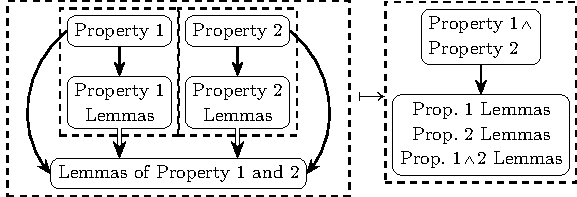
\includegraphics{graphproperty.pdf}
\caption{Combining plugins}\label{fig:properties}
\end{figure}

We use Coq's typeclass system to manage our plugins smoothly, essentially to enable the diagram in Figure~\ref{fig:properties}.  The idea is that if we have two properties, each of which come with some already-proved lemmas, we can combine these plugins to prove the emergent lemmas that result from the combination, and then treat the new combination as a new plugin, \emph{i.e.} the system is compositional.  For example, we compose \p{BiGraph}, \p{MathGraph}, and \p{FiniteGraph} together into a new plugin we call \p{BiMaFin}.  \p{BiMaFin} is the actual soundness condition used to verify the program in Figure~\ref{fig:markgraph}.

%% We can apply our framework to define related structures such as DAGs and trees.
%% For example, a DAG has the additional property that for any $x$ and $y$,
%% if $x$ is reachable from $y$, then $x = y$ or $y$ is not reachable
%% from $x$.
%  Similarly, we define tree by saying that for any reachable node $n$ there is
%a unique path from the root to $n$.

\subsection{Reasoning about relations between graphs} %Using our framework to reasonApplication of the framework}

In Figure~\ref{fig:markgraph} we defined the relation $\m{mark}(\gamma, \tx x, \gamma')$
for the graph marking algorithm.  Similarly, we define $\m{span}$ for the spanning tree program
and $\m{copy}$ for the graph copy program.
These relations all capture how the graph has changed from before to after the program
execution.  By specifying $\m{copy}$ relationally
rather than functionally we avoid explicitly modeling how the memory allocator works, a major advantage.

As previously mentioned, we reuse $\m{mark}$ and its
related lemmas to prove facts about spanning tree and graph copy
because the latter two programs mark nodes as they work.
Accordingly, we can reuse facts such as the following:
%%%%%%%%%%%%%%%%%%%%%%%%%%%%%%%%%%%%%%%%%%%%%%%%%%
%%%%%% Edit 4
%%%%%%%%%%%%%%%%%%%%%%%%%%%%%%%%%%%%%%%%%%%%%%%%%%
%%%%%%%%%%%%%%%%%%%%%%%%%%%%%%%%%%%%%%%%%%%%%%%%%%
%%%%%% Edit 4: Qinxiang's proposal starts
%%%%%%%%%%%%%%%%%%%%%%%%%%%%%%%%%%%%%%%%%%%%%%%%%%
\[
\begin{array}{@{}l@{}}
\text{if } \gamma(x)=(0, v_1, \dots,v_n), \m{mark1}(\gamma, x, \gamma_1), \\
\text{and } \forall i, \m{mark}(\gamma_i,v_i,\gamma_{i+1}) \text{ then } \m{mark}(\gamma,x,\gamma_{n+1}).
\end{array}
\]
%We prove this theorem sound for any LabeledGraph, not just
%\p{BiGraph}s (\emph{i.e.}, we do not assume only two neighbors).
%%%%%%%%%%%%%%%%%%%%%%%%%%%%%%%%%%%%%%%%%%%%%%%%%%
%%%%%% Edit 4: Qinxiang's proposal ends
%%%%%%%%%%%%%%%%%%%%%%%%%%%%%%%%%%%%%%%%%%%%%%%%%%


